\documentclass[12pt,a4paper]{article}

% ─── Page Layout ───────────────────────────────────────────────────────────────
\usepackage[a4paper, margin=0.8in, headheight=14pt]{geometry}

% ─── Fonts (XeLaTeX) ───────────────────────────────────────────────────────────
\usepackage{fontspec}
\usepackage{unicode-math}
\setmainfont{TeX Gyre Pagella}
\setmonofont[Scale=0.88]{TeX Gyre Cursor}
\setmathfont{Latin Modern Math}

% ─── Packages ──────────────────────────────────────────────────────────────────
\usepackage{xcolor}
\usepackage{colortbl}
\usepackage{titlesec}
\usepackage{enumitem}
\usepackage{tabularx}
\usepackage{booktabs}
\usepackage{array}
\usepackage{amsmath}
\usepackage{tikz}
\usetikzlibrary{shapes.geometric, arrows.meta, positioning, calc, fit, decorations.pathreplacing}
\usepackage{tcolorbox}
\tcbuselibrary{skins, breakable}
\usepackage{hyperref}
\usepackage{fancyhdr}
\usepackage{graphicx}
\usepackage{microtype}
\hyphenpenalty=10000
\exhyphenpenalty=10000
\sloppy
\usepackage{caption}
\usepackage{setspace}
\usepackage{multirow}
\usepackage{tocloft}

% ─── Q&A helper ────────────────────────────────────────────────────────────────
\newcommand{\Q}[1]{\textbf{#1}\par\noindent\ignorespaces}

% ─── Colour Palette ────────────────────────────────────────────────────────────
\definecolor{myred}{RGB}{196,30,58}
\definecolor{mydark}{RGB}{30,30,50}
\definecolor{mygreen}{RGB}{14,120,80}
\definecolor{myteal}{RGB}{0,130,140}
\definecolor{myamber}{RGB}{180,100,0}
\definecolor{mypurple}{RGB}{100,30,160}
\definecolor{mygray}{RGB}{246,247,249}
\definecolor{mgframe}{RGB}{180,185,200}
\definecolor{watermark}{RGB}{145,150,170}
\definecolor{hdrred}{RGB}{250,232,235}
\definecolor{hdrgreen}{RGB}{220,244,233}
\definecolor{hdrteal}{RGB}{220,242,244}
\definecolor{hdramber}{RGB}{253,242,215}
\definecolor{hdrpurple}{RGB}{238,228,255}
\definecolor{hdrgray}{RGB}{238,240,245}
\definecolor{rowalt}{RGB}{250,251,253}

% ─── Section Formatting ────────────────────────────────────────────────────────
\titleformat{\section}
  {\large\bfseries\color{myred}}{\thesection.}{0.5em}{}
  [\vspace{1pt}{\color{myred}\rule{\linewidth}{0.8pt}}]
\titleformat{\subsection}
  {\normalsize\bfseries\color{myteal}}{\thesubsection}{0.5em}{}
\titlespacing*{\section}{0pt}{18pt}{7pt}
\titlespacing*{\subsection}{0pt}{11pt}{4pt}

% ─── Paragraph ─────────────────────────────────────────────────────────────────
\setlength{\parindent}{0pt}
\setlength{\parskip}{4pt}

% ─── TOC Styling ───────────────────────────────────────────────────────────────
\renewcommand{\cfttoctitlefont}{\large\bfseries\color{myred}}
\renewcommand{\cftaftertoctitle}{\par\noindent{\color{myred}\rule{\linewidth}{0.8pt}}}
\setlength{\cftbeforetoctitleskip}{0pt}
\setlength{\cftaftertoctitleskip}{6pt}
\renewcommand{\cftsecfont}{\normalsize\bfseries\color{mydark}}
\renewcommand{\cftsecpagefont}{\normalsize\bfseries\color{mydark}}
\renewcommand{\cftsecleader}{\cftdotfill{\cftdotsep}}
\setlength{\cftbeforesecskip}{7pt}
\renewcommand{\cftsubsecfont}{\small\color{mydark}}
\renewcommand{\cftsubsecpagefont}{\small\color{mydark}}
\setlength{\cftbeforesubsecskip}{3pt}
\setlength{\cftsubsecindent}{1.4em}

% ─── Table helpers ─────────────────────────────────────────────────────────────
\renewcommand{\arraystretch}{1.45}
\setlength{\tabcolsep}{6pt}
\arrayrulecolor{mydark}
\newcolumntype{B}[1]{>{\small\bfseries\raggedright\arraybackslash}m{#1}}
\newcolumntype{Y}{>{\small\raggedright\arraybackslash}X}
\renewcommand{\tabularxcolumn}[1]{m{#1}}

% ─── Header / Footer ───────────────────────────────────────────────────────────
\pagestyle{fancy}
\fancyhf{}
\fancyhead[L]{\small\color{myred}\textbf{OE-EC704B}\;\color{mydark}--- Optimization Technique}
\fancyhead[R]{\small\color{myteal}\textbf{Module 3 Notes}}
\fancyfoot[C]{\small\color{mydark}\thepage}
\fancyfoot[R]{\small\color{watermark}\textit{\copyright\ Biraj}}
\renewcommand{\headrulewidth}{0.5pt}
\renewcommand{\footrulewidth}{0.3pt}

% ─── Hyperref ──────────────────────────────────────────────────────────────────
\hypersetup{
  colorlinks=true, linkcolor=myteal, urlcolor=myteal,
  pdfauthor={Biraj Sarkar},
  pdftitle={OE-EC704B --- Module 3 Notes}
}

% ─── tcolorbox styles ──────────────────────────────────────────────────────────
\tcbset{
  tikzbox/.style={
    colback=mygray, colframe=mgframe, boxrule=0.6pt, arc=4pt,
    left=8pt, right=8pt, top=6pt, bottom=6pt,
    colbacktitle=mgframe, coltitle=mydark,
    fonttitle=\small\bfseries
  },
  defbox/.style={
    colback=hdrgreen, colframe=mygreen, boxrule=0.8pt, arc=4pt,
    left=9pt, right=9pt, top=6pt, bottom=6pt,
    colbacktitle=mygreen, coltitle=white,
    fonttitle=\small\bfseries
  },
  formulabox/.style={
    colback=hdrteal, colframe=myteal, boxrule=0.8pt, arc=4pt,
    left=9pt, right=9pt, top=7pt, bottom=7pt,
    colbacktitle=myteal, coltitle=white,
    fonttitle=\small\bfseries
  },
  examplebox/.style={
    colback=hdramber, colframe=myamber, boxrule=0.8pt, arc=4pt,
    left=9pt, right=9pt, top=6pt, bottom=6pt,
    colbacktitle=myamber, coltitle=white,
    fonttitle=\small\bfseries
  },
  masonbox/.style={
    colback=hdrpurple, colframe=mypurple, boxrule=0.8pt, arc=4pt,
    left=9pt, right=9pt, top=6pt, bottom=6pt,
    colbacktitle=mypurple, coltitle=white,
    fonttitle=\small\bfseries
  },
  exambox/.style={
    colback=hdrpurple, colframe=mypurple, boxrule=1pt, arc=5pt,
    left=10pt, right=10pt, top=8pt, bottom=8pt,
    colbacktitle=mypurple, coltitle=white,
    fonttitle=\bfseries,
    breakable, title after break={\textbf{Frequently Asked / Viva Questions (contd.)}}}
}
\tcbset{breakable}

% ─── TikZ styles ───────────────────────────────────────────────────────────────
\tikzset{
  block/.style={rectangle, draw=myteal, fill=hdrteal,
    text width=2.4cm, align=center, minimum height=0.95cm,
    font=\small, rounded corners=3pt, line width=0.7pt},
  redblock/.style={rectangle, draw=myred, fill=hdrred,
    text width=2.4cm, align=center, minimum height=0.95cm,
    font=\small, rounded corners=3pt, line width=0.7pt},
  netnode/.style={rectangle, draw=myteal, fill=hdrteal,
    text width=1.5cm, align=center, minimum height=0.8cm,
    font=\small, rounded corners=3pt, line width=0.7pt},
  sumjunc/.style={circle, draw=myamber, fill=hdramber,
    minimum size=0.62cm, font=\small, line width=0.8pt},
  snode/.style={circle, draw=mypurple, fill=hdrpurple,
    minimum size=0.55cm, font=\footnotesize, line width=0.7pt},
  arrow/.style={-Stealth, thick, color=mydark},
  redarrow/.style={-Stealth, thick, color=myred},
  line/.style={thick, color=mydark}
}

% ═══════════════════════════════════════════════════════════════════════════════
\begin{document}
% ═══════════════════════════════════════════════════════════════════════════════

\begin{center}
  {\LARGE\bfseries\color{myred} OE-EC704B --- Optimization Technique}\\[5pt]
  {\normalsize\color{mydark} Semester VII \quad$\bullet$\quad 3L:0T:0P \quad$\bullet$\quad 3 Credits}\\[3pt]
  {\normalsize\color{myteal}\textbf{Module 3 Exam Notes: Gradient-Based Methods}}\\[3pt]
  {\small\color{mydark} CGEC \;$|$\; B.Tech ECE (2023--27) \;$|$\; \textit{Biraj Sarkar}}
\end{center}
\vspace{2pt}
\noindent{\color{myred}\rule{\linewidth}{1.5pt}}
\vspace{2pt}

\hypersetup{linkcolor=mydark}
\tableofcontents
\hypersetup{linkcolor=myteal}
\newpage

% ===============================================================================
\section{Fundamentals of Gradient-Based Search}
% ===============================================================================

Gradient-based single-variable methods use derivative information to find stationary points by solving:
\begin{equation}
  g(x) = f'(x) = 0
\end{equation}
These algorithms are highly efficient because derivatives provide the slope and curvature of the objective function, indicating the direction and distance to the optimum.

% ===============================================================================
\section{Newton-Raphson Method}
% ===============================================================================

The Newton-Raphson method is a second-order method that approximates the function locally with a quadratic Taylor series expansion.

\subsection{Derivation of the Iterative Formula}
Let $x_k$ be the current estimate of the optimum. Expanding the first derivative $f'(x)$ about $x_k$ using a first-order Taylor series yields:
\begin{equation*}
  f'(x) \approx f'(x_k) + f''(x_k)(x - x_k)
\end{equation*}
To locate the stationary point ($x_{k+1}$ where $f'(x_{k+1}) = 0$):
\begin{equation*}
  f'(x_k) + f''(x_k)(x_{k+1} - x_k) = 0
\end{equation*}
Rearranging for $x_{k+1}$ gives the standard \textbf{Newton-Raphson Update}:

\begin{tcolorbox}[formulabox, title={Newton-Raphson Iterative Equation}]
\begin{equation}
  x_{k+1} = x_k - \frac{f'(x_k)}{f''(x_k)}
\end{equation}
Where:
\begin{itemize}[leftmargin=*, itemsep=2pt, topsep=0pt]
  \item $f'(x_k)$ is the first derivative (slope) at step $k$.
  \item $f''(x_k)$ is the second derivative (curvature) at step $k$.
\end{itemize}
\end{tcolorbox}

\subsection{Convergence and Characteristics}
\begin{itemize}[leftmargin=*, itemsep=2.5pt]
  \item \textbf{Quadratic Convergence:} Near the optimum, the error decreases quadratically ($e_{k+1} \propto e_k^2$), making it the fastest gradient-based method.
  \item \textbf{Limitations:} Requires computing the analytical second derivative $f''(x)$. If $f''(x_k) = 0$, the method fails. It is highly sensitive to the initial guess $x_0$ and can diverge if starting far from the root.
\end{itemize}

\begin{tcolorbox}[tikzbox, title={Graphical projection of Newton-Raphson}]
\centering
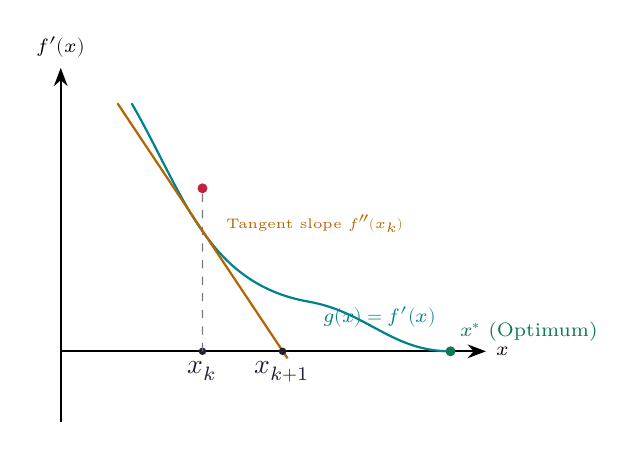
\begin{tikzpicture}[scale=0.9]
  % Draw axes
  \draw[-Stealth, thick] (0,0) -- (6,0) node[right, font=\scriptsize\bfseries] {$x$};
  \draw[-Stealth, thick] (0,-1) -- (0,4) node[above, font=\scriptsize\bfseries] {$f'(x)$};
  
  % Draw curve f'(x)
  \draw[thick, color=myteal] (1,3.5) to[out=-60, in=170] (3.5,0.7) to[out=-10, in=180] (5.5,0);
  \node[above, font=\scriptsize\color{myteal}] at (4.5,0.2) {$g(x) = f'(x)$};

  % Tangent at x_k
  \coordinate (xk) at (2.0,2.3);
  \fill[mydark] (2.0,0) circle (1.5pt) node[below] {$x_k$};
  \fill[myred] (xk) circle (2pt);
  \draw[dashed, color=mydark!60] (2.0,0) -- (xk);
  
  % Tangent line: y - 2.3 = m*(x - 2) -> hits zero at x_k+1
  \draw[thick, color=myamber] (0.8,3.5) -- (3.2,-0.1);
  \node[right, font=\tiny, color=myamber] at (2.2,1.8) {Tangent slope $f''(x_k)$};
  
  % Projections
  \coordinate (xkp1) at (3.13,0);
  \fill[mydark] (xkp1) circle (1.5pt) node[below] {$x_{k+1}$};
  \fill[mygreen] (5.5,0) circle (2pt) node[above right, font=\scriptsize] {$x^*$ (Optimum)};
\end{tikzpicture}
\end{tcolorbox}

% ===============================================================================
\section{Bisection Method}
% ===============================================================================

The bisection method is a robust first-order bracketing technique that solves $f'(x) = 0$ by halving intervals based on sign changes.

\begin{tcolorbox}[defbox, title={Bisection Criterion}]
Let the initial interval be $[a, b]$. If $f'(x)$ is continuous and:
\begin{equation}
  f'(a) \cdot f'(b) < 0
\end{equation}
then by the Intermediate Value Theorem, at least one stationary point $x^*$ exists in $[a, b]$ where $f'(x^*) = 0$.
\end{tcolorbox}

\subsubsection{Algorithm Steps}
\begin{enumerate}[label=\textbf{\arabic*.}, leftmargin=*, itemsep=2.5pt]
  \item Calculate the midpoint: $x_0 = \frac{a+b}{2}$ and evaluate $f'(x_0)$.
  \item If $|f'(x_0)| \le \epsilon$ (tolerance), stop; $x^* \approx x_0$.
  \item If $f'(a) \cdot f'(x_0) < 0$, the root lies in $[a, x_0]$. Set $b = x_0$.
  \item If $f'(x_0) \cdot f'(b) < 0$, the root lies in $[x_0, b]$. Set $a = x_0$.
  \item Repeat until $|b-a| \le \epsilon$. Convergence is guaranteed, though linear and slow.
\end{enumerate}

% ===============================================================================
\section{Secant Method}
% ===============================================================================

The secant method approximates the second derivative $f''(x)$ in the Newton-Raphson formula using two previous evaluations, avoiding analytical differentiation.

\subsection{Iterative Formula}
The curvature is approximated using finite differences between $x_k$ and $x_{k-1}$:
\begin{equation}
  f''(x_k) \approx \frac{f'(x_k) - f'(x_{k-1})}{x_k - x_{k-1}}
\end{equation}
Substituting this into the Newton equation yields the \textbf{Secant Iterative Update}:

\begin{tcolorbox}[formulabox, title={Secant Method Equation}]
\begin{equation}
  x_{k+1} = x_k - f'(x_k) \left[ \frac{x_k - x_{k-1}}{f'(x_k) - f'(x_{k-1})} \right]
\end{equation}
This method requires two initial guess points $x_0$ and $x_1$, and converges superlinearly with a convergence rate of:
\begin{equation}
  \text{Rate } \approx 1.618
\end{equation}
\end{tcolorbox}

% ===============================================================================
\section{Computer Programs / Pseudo-Codes}
% ===============================================================================

\begin{tcolorbox}[tikzbox, title={Newton-Raphson Optimization Pseudo-code}]
\begin{spacing}{1.1}
\begin{verbatim}
Input: Initial guess x0, tolerance eps, max_iter
Output: Local minimum coordinate x*

Function NewtonRaphson(x0, eps, max_iter):
    x = x0
    For k = 1 to max_iter:
        df = FirstDerivative(x)
        ddf = SecondDerivative(x)
        If |ddf| < 1e-12: 
            Print "Error: Curvature close to zero!"
            Return null
        x_new = x - df / ddf
        If |x_new - x| < eps or |df| < eps:
            Return x_new
        x = x_new
    Return x
\end{verbatim}
\end{spacing}
\end{tcolorbox}

\begin{tcolorbox}[tikzbox, title={Secant Optimization Pseudo-code}]
\begin{spacing}{1.1}
\begin{verbatim}
Input: Two initial guesses x0, x1, tolerance eps, max_iter
Output: Local minimum coordinate x*

Function SecantMethod(x0, x1, eps, max_iter):
    x_prev = x0
    x_curr = x1
    For k = 1 to max_iter:
        df_prev = FirstDerivative(x_prev)
        df_curr = FirstDerivative(x_curr)
        If |df_curr - df_prev| < 1e-12:
            Print "Error: Denominator is zero!"
            Return null
        x_next = x_curr - df_curr * (x_curr - x_prev) / (df_curr - df_prev)
        If |x_next - x_curr| < eps:
            Return x_next
        x_prev = x_curr
        x_curr = x_next
    Return x_curr
\end{verbatim}
\end{spacing}
\end{tcolorbox}

\newpage

% ===============================================================================
% MANDATORY QUICK REVISION PAGE
% ===============================================================================
\begin{center}
  {\large\bfseries\color{myred} Quick Revision --- Module 3}\\[3pt]
  {\small\color{mydark} Gradient-Based Methods $|$ OE-EC704B}
\end{center}
\noindent{\color{myred}\rule{\linewidth}{1.2pt}}
\vspace{4pt}

\begin{tcolorbox}[formulabox, title={\textbf{Key Formulas \& Convergence Rates}}]
\renewcommand{\arraystretch}{1.45}
\begin{tabularx}{\linewidth}{B{5.0cm} X}
Newton-Raphson Formula & $x_{k+1} = x_k - \frac{f'(x_k)}{f''(x_k)}$. \\[4pt]
Newton Convergence & Quadratic rate: $e_{k+1} \approx C e_k^2$. \\[4pt]
Bisection Condition & $f'(a) \cdot f'(b) < 0$ \quad (signs must be opposite). \\[4pt]
Secant Update Formula & $x_{k+1} = x_k - f'(x_k) \left[ \frac{x_k - x_{k-1}}{f'(x_k) - f'(x_{k-1})} \right]$. \\[4pt]
Secant Convergence & Superlinear rate: $e_{k+1} \approx C e_k^{1.618}$. \\
\end{tabularx}
\end{tcolorbox}

\begin{tcolorbox}[defbox, title={\textbf{One-Line Definitions}}]
\begin{itemize}[leftmargin=*, itemsep=2.5pt, topsep=0pt]
  \item \textbf{Gradient-Based Optimization:} Minimizing/maximizing functions using directional slope (derivatives) rather than search comparisons alone.
  \item \textbf{Newton-Raphson Method:} An iterative root-finding technique using tangent lines to estimate the point where the derivative is zero.
  \item \textbf{Bisection Method:} A root-finding algorithm that repeatedly bisects an interval and selects a sub-interval in which a sign change occurs.
  \item \textbf{Secant Method:} A gradient-based optimization method that replaces analytical second derivatives with finite difference slope approximations.
  \item \textbf{Quadratic Convergence:} A convergence behavior where the number of correct decimal places roughly doubles with each iteration.
  \item \textbf{Intermediate Value Theorem:} Theorem stating that if a continuous function has opposite signs at interval boundaries, it must cross zero inside.
\end{itemize}
\end{tcolorbox}

\begin{tcolorbox}[exambox, title={\textbf{Frequently Asked / Viva Questions}}]
\begin{enumerate}[topsep=0pt, label=\textbf{Q\arabic*.}, itemsep=5pt]
  \item \Q{Compare Newton-Raphson and Secant methods based on derivative requirements.}
    Newton-Raphson requires evaluating both the first derivative $f'(x)$ and the analytical second derivative $f''(x)$ at each step. The Secant method only requires the first derivative $f'(x)$ because it approximates $f''(x)$ using finite differences.
  \item \Q{State the convergence rate of the Newton-Raphson method and define what it means.}
    It converges quadratically ($e_{k+1} \propto e_k^2$). This means the error in step $k+1$ is proportional to the square of the error in step $k$, leading to extremely rapid convergence near the root.
  \item \Q{Why does the Newton-Raphson method fail if $f''(x_k) = 0$?}
    Because the formula involves dividing by the second derivative. If $f''(x_k) = 0$, the tangent to $f'(x)$ becomes parallel to the x-axis, and the projection point $x_{k+1}$ moves to infinity (division by zero error).
  \item \Q{Explain the role of the sign check $f'(a) \cdot f'(b) < 0$ in the Bisection method.}
    It guarantees that the first derivative $f'(x)$ changes sign across the interval $[a, b]$. For a continuous derivative, this ensures that at least one stationary point (root of $f'(x)=0$) lies within the interval.
  \item \Q{What are the primary disadvantages of the Bisection method?}
    It has a slow, linear convergence rate. It does not utilize the magnitude of the derivative, only its sign, making it take many iterations compared to Newton's method.
  \item \Q{Write down the Secant method update equation.}
    $x_{k+1} = x_k - f'(x_k) \left[ \frac{x_k - x_{k-1}}{f'(x_k) - f'(x_{k-1})} \right]$.
  \item \Q{How does the Secant method differ from the regular False Position (Regula Falsi) root-finding method?}
    False Position always brackets the root and retains points of opposite signs. The Secant method simply uses the last two calculated points, meaning it is not guaranteed to bracket the root and can occasionally diverge.
  \item \Q{What is the convergence rate of the Secant method?}
    It converges superlinearly with order $\alpha = \frac{1+\sqrt{5}}{2} \approx 1.618$ (the Golden Ratio).
  \item \Q{Under what conditions can the Newton-Raphson method diverge?}
    It can diverge if the initial guess $x_0$ is chosen far from the optimum, especially in regions with inflection points, local extrema of $f'(x)$, or flat regions where $f''(x) \approx 0$.
  \item \Q{Write a short MATLAB/Python routine snippet for updating the Secant point.}
    \verb|x_next = x_curr - df_curr * (x_curr - x_prev) / (df_curr - df_prev)| where \verb|df| is the derivative function.
\end{enumerate}
\end{tcolorbox}

\end{document}
